\documentclass[10pt,a4paper]{ctexart}
\usepackage[margin=2.5cm]{geometry}
\usepackage[utf8]{inputenc}
\usepackage{amsmath}
\usepackage{amsfonts}
\usepackage{amssymb}
\usepackage{epsfig}
\usepackage{ifthen}
\usepackage{multicol}

%\newlength{\la}
%\newlength{\lb}
%\newlength{\lc}
%\newlength{\ld}
%\newlength{\lhalf}
%\newlength{\lquarter}
%\newlength{\lmax}
\newcommand{\xx}[4]{\\[.5pt]%
	\settowidth{\la}{A.~#1~~~}
	\settowidth{\lb}{B.~#2~~~}
	\settowidth{\lc}{C.~#3~~~}
	\settowidth{\ld}{D.~#4~~~}
	\ifthenelse{\lengthtest{\la > \lb}} {\setlength{\lmax}{\la}} {\setlength{\lmax}{\lb}}
	\ifthenelse{\lengthtest{\lmax < \lc}} {\setlength{\lmax}{\lc}} {}
	\ifthenelse{\lengthtest{\lmax < \ld}} {\setlength{\lmax}{\ld}} {}
	\setlength{\lhalf}{0.5\linewidth}
	\setlength{\lquarter}{0.25\linewidth}
	\ifthenelse{\lengthtest{\lmax > \lhalf}} {\noindent{}A.~#1 \\ B.~#2 \\ C.~#3 \\ D.~#4 } {
		\ifthenelse{\lengthtest{\lmax > \lquarter}} {\noindent\makebox[\lhalf][l]{A.~#1~~~}%
			\makebox[\lhalf][l]{B.~#2~~~}\par%
			\makebox[\lhalf][l]{C.~#3~~~}%
			\makebox[\lhalf][l]{D.~#4~~~}}%
		{\noindent\makebox[\lquarter][l]{A.~#1~~~}%
			\makebox[\lquarter][l]{B.~#2~~~}%
			\makebox[\lquarter][l]{C.~#3~~~}%
			\makebox[\lquarter][l]{D.~#4~~~}}}}
\newcommand{\xz}[1][1]{\nolinebreak\mbox{(\hspace{1cm})}\\\vspace{-0.33cm}}
\newcommand{\tk}[1][2.5]{\,\underline{\mbox{\hspace{#1 cm}}}\,}

\usepackage{setspace}

\usepackage{graphics}
\usepackage{float}
\usepackage{caption,subcaption}


\pagestyle{plain}
\title{\Large{\textbf{2022年全国高中数学联合竞赛一试B卷}}}
\date{2022年9月11日}
\author{制卷单位:江苏省数学学会}
%\author{学校\underline{\hspace{3cm}}姓名\underline{\hspace{3cm}} 城市\underline{\hspace{3cm}}}

\begin{document}
	\maketitle
	\subsection*{考生须知}
	\begin{enumerate}
		\item 答卷前,考生务必将自己的姓名和准考证号填写在答题卡上。
		\item 考试结束后,将本试卷和答题卡一并交回。
	\end{enumerate}
	请认真核对监考员在答题卡上所粘贴的条形码上的姓名、准考证号与您本人是否相符。	
	\subsection*{一、填空题,本大题共8小题,每小题8分,满分64分.}
	\begin{spacing}{1.8}
		\begin{itemize}
			\item[1.] 不等式$\frac{20}{x-9}>\frac{22}{x-11}$的解集为\tk.
			\item[2.] 在平面直角坐标系中, 以抛物线$\Gamma :y^2=6x$为焦点为圆心作一个圆$\Omega$,与$\Gamma$的准线相切,则圆$\Omega$的面积为\tk.
			\item[3.] 函数$f(x)=\lg{2} \cdot \lg{5}-\lg{2x} \cdot \lg{5x}$的最大值为\tk. 
			\item[4.] 一枚不均匀的硬币, 若随机抛掷它两次均得到正面的概率为$\frac{1}{2}$, 则随机抛掷它两次得到正面、反面各一次的概率为\tk.
			\item[5.] 已知复数z满足$|z|=1$,且$Re\frac{z+1}{\bar{z}+1}=\frac{1}{3}$,则$Re\frac{z}{\bar{z}}$的值为\tk.
			\item[6.] 若正四棱雉$P-ABCD$的各条棱长均相等,$M$为棱$AB$的中点, 则异面直线$BP$与$CM$所成的角的余弦值为\tk.
			\item[7.] 若$\Delta ABC$的三个内角$A,B,C$满足$\cos{A}=\sin{B}=2\tan{\frac{C}{2}}$,则$\sin{A}+\cos{A}+2\tan{A}$的值为\tk.
			\item[8.]一个单位方格的四条边中, 若存在三条边染了三种不同的颜色, 则称该单位方格是 “多彩”的. 如图, 一个$1 \times 3$方格表的表格线共含 10 条单位长线段, 现要对这 10 条线段染色, 每条线段染为红、黄、蓝三色之一,使得三个单位方格都是"多彩"的.这样的染色方式数为\tk(答案用数值表示).
			\begin{center}
				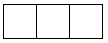
\includegraphics[width=0.2\textwidth]{tkt1.png}
			\end{center} 
		\end{itemize}
	\end{spacing}
	\newpage
	
	\subsection*{三、简答题, 本大题共3小题,满分56分.解答应写出文字说明、证明过程或演算步骤.}
	\begin{spacing}{1.8}
		\begin{itemize}
			\item[9.](本题满分16分)在平面直角坐标系中,$F_1,F_2$是双曲线$\Gamma :\frac{x^2}{3}-y^2=1$的两个焦点,$\Gamma$上一点$P$满足$\vec{PF_1} \cdot \vec{PF_2}=1$.求点$P$到$\Gamma$的两条渐近线距离之和.
			\item[10.](本题满分20分)设正数$a_1,a_2,a_3,b_1,b_2,b_3$满足:$a_1,a_2,a_3$成公差为$b_1$的等差数列,$b_1,b_2,b_3$成公比$a_1$的等差数列,且$a_3=b_3$.求$a_3$的最小值,并确定当$a_3$取到最小值时$a_1,a_2$的值.
			\item[11.](本题满分20分)若$a,b$为实数,$a<b$,函数$y=\sin{x}$在闭区间$[a,b]$上的最大值与最小值之差为1,$b-a$的取值范围.
		\end{itemize}
	\end{spacing}
\end{document}